\clearpage
\section{Analyzing the \ourdataset \ Dataset}
\label{sec:dataset_details}

\begin{wraptable}[12]{r}{0.5\textwidth}
\vspace{-0.4cm}
\caption{Breakdown of source news articles by news outlet.}
\vspace{-0.25cm}
\resizebox{\linewidth}{!}{
\begin{tabular}{lc}
\toprule
\textbf{Source} & \textbf{Articles (\%Total)} \\
\midrule
Forbes & 110,103 (44.3\%) \\
The Hindustan Times & \ 80,000 \ (32.2\%) \\ 
The Irish Times & \ 29,546 \  (11.9\%) \\ 
Deutsche Welle (DW) & \ 21,317 \ (8.6\%) \\ 
Cable News Net (CNN) & \ \ 7,355 \ \  (3.0\%) \\ \midrule
\textbf{Total} & \ \textbf{248,321 (100\%)} \\
\bottomrule
\end{tabular}}
\vspace{-0.3cm}
\label{tab:dist}
\end{wraptable}
\textbf{News Corpus Details.} We drew from a heterogeneous pool of news articles diversified by geography, time, and topic to ensure broad coverage. We collected a English-language articles from outlets including Forbes, Hindustan Times, The Irish Times, Deutsche Welle, and CNN. They were selected by first collecting a corpus of approximately 250,000 articles spanning from June 2023 to April 2025, encompassing major large-scale events across sports, geopolitics, local news, crime, entertainment, and the arts. Then, performing de-duplication and filtering for language, text availability, and valid dates, we retained approximately 248,000 articles for the question generation phase. Table \ref{tab:dist} details the distribution across news outlets for our corpus. 


The overall dataset creation process costed us ~3000\$ with training set costing ~2200\$ (using DeepSeek-v3) while creating the test set costed ~800\$ (using o4-mini-high and grok-4.1-fast with search tool). 


\vspace{0.15cm}

\subsection{Analysis of Best Question Selection}


\begin{figure}[h]
\begin{minipage}{0.55\textwidth}
\resizebox{\linewidth}{!}{
\centering
    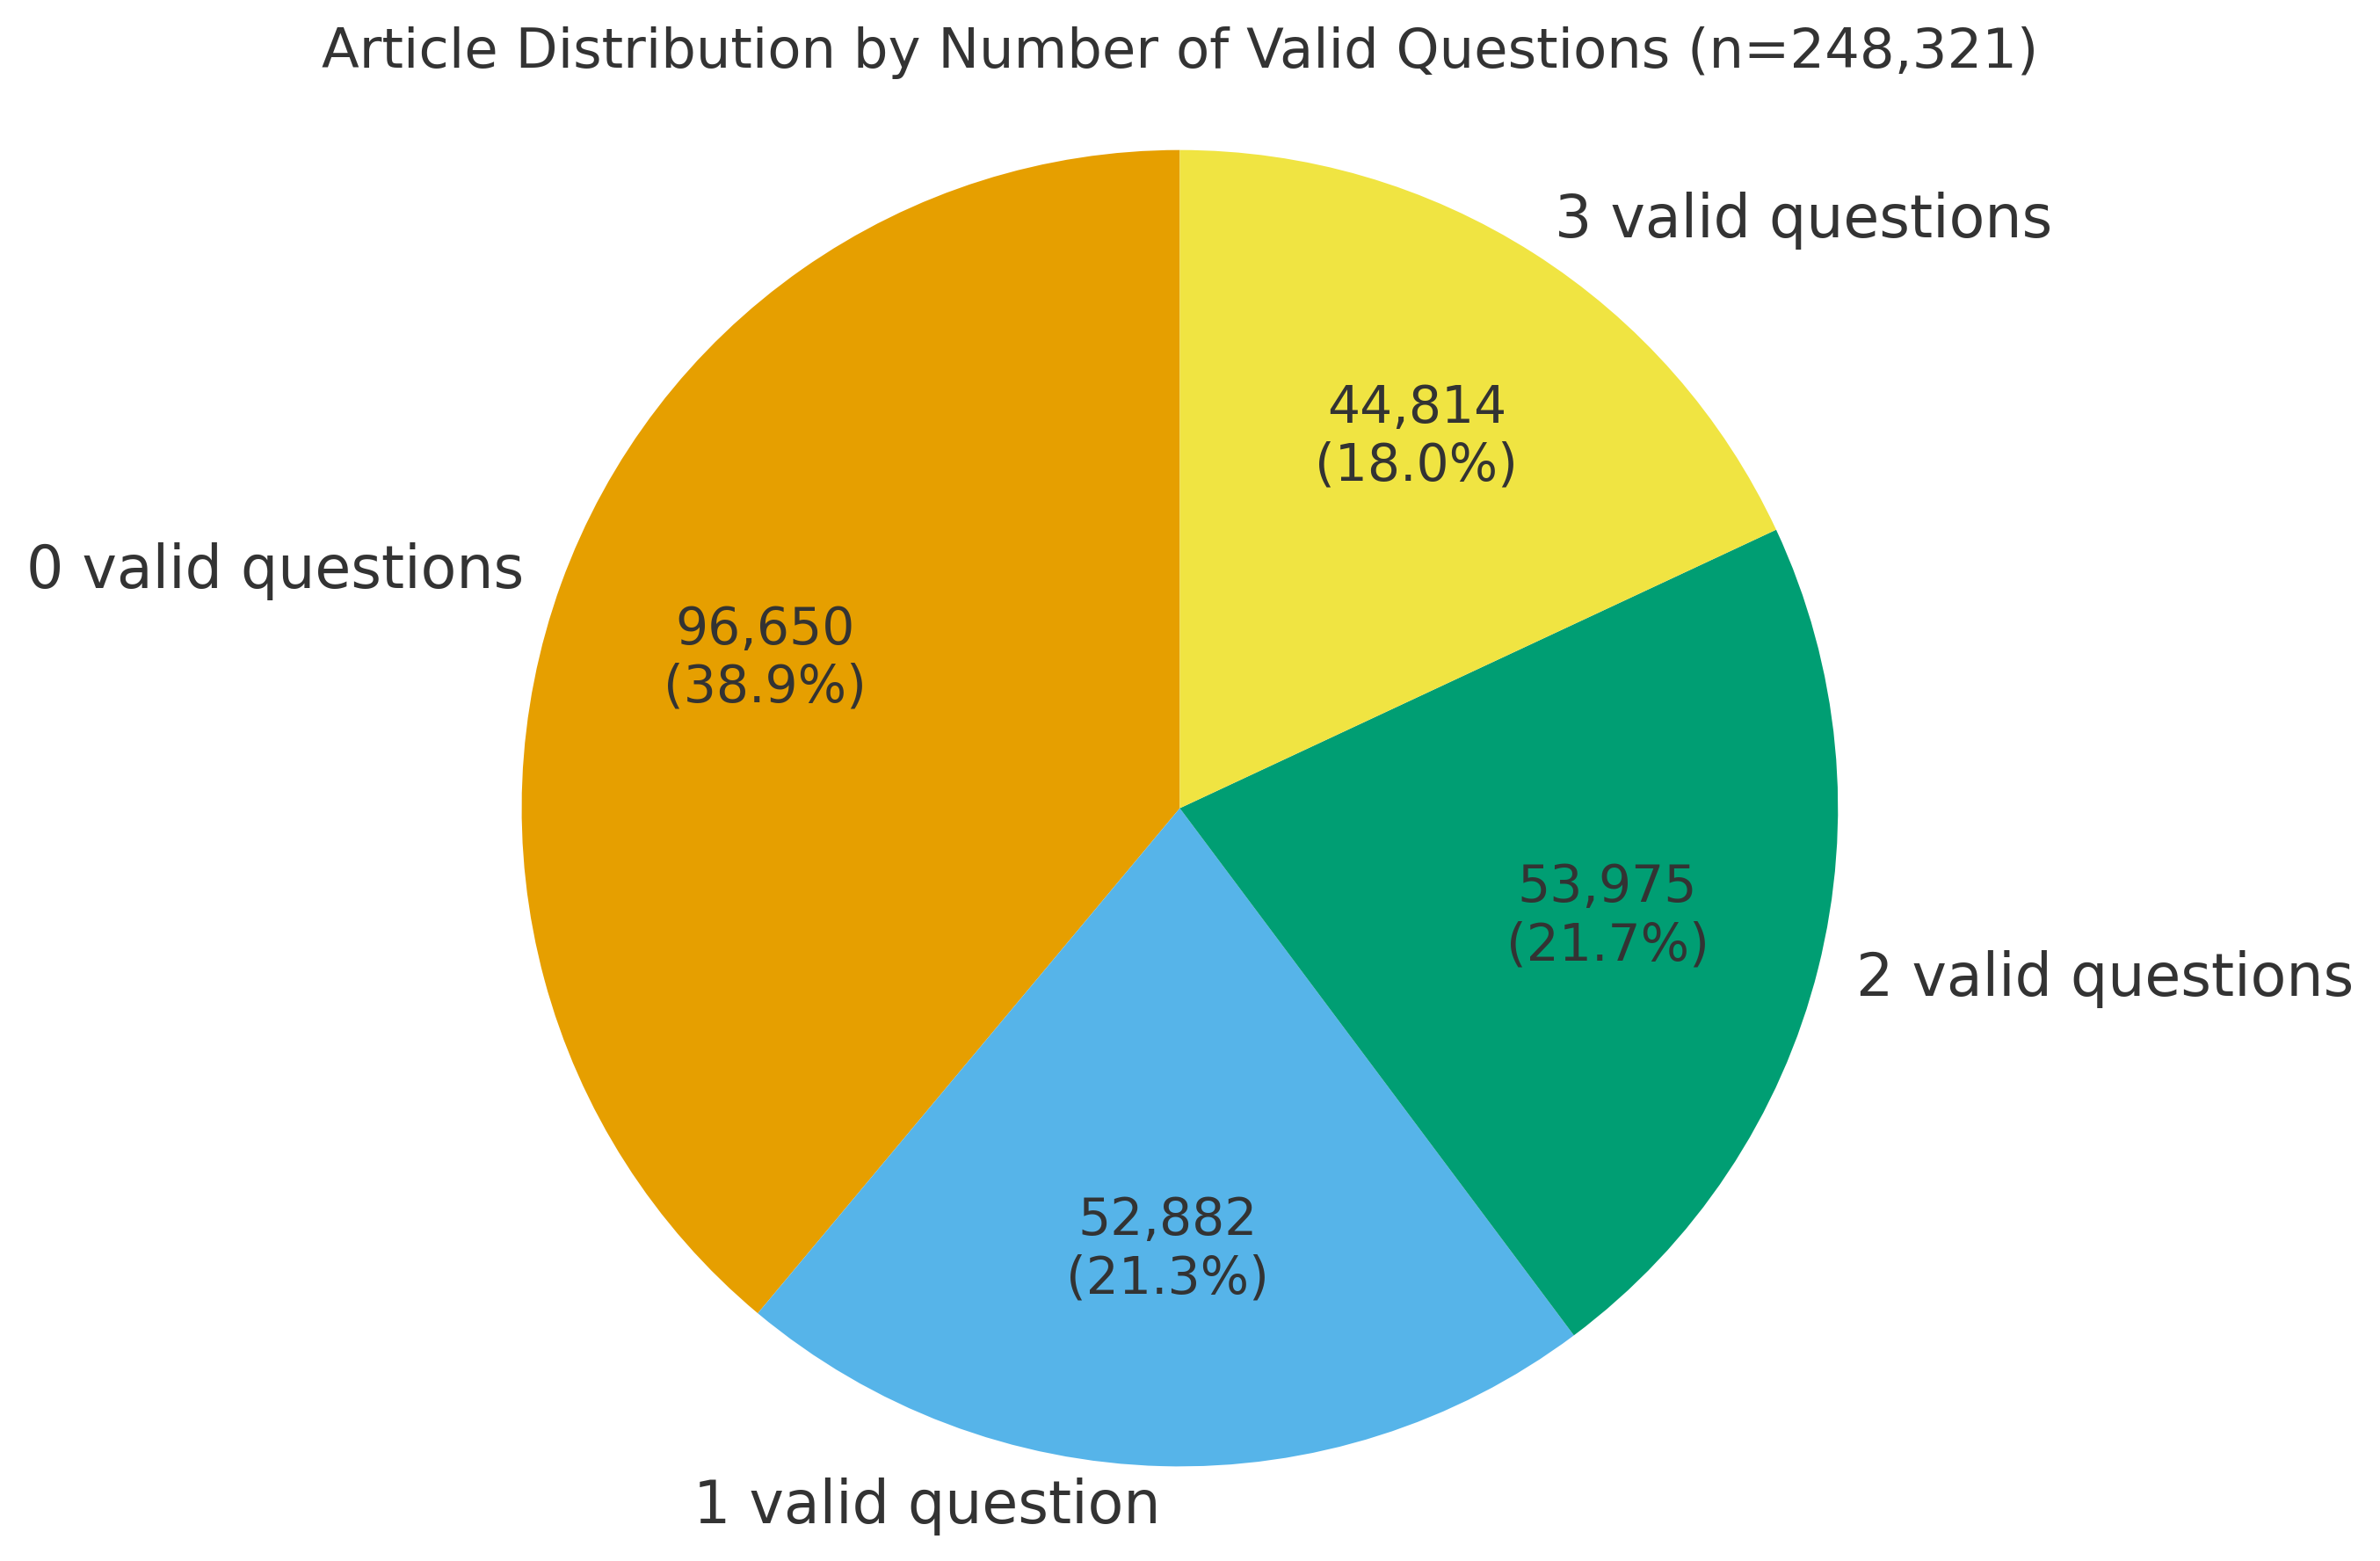
\includegraphics[]{figures/pie_chart.png}}
    \end{minipage}
    \hfill
\begin{minipage}{0.41\textwidth}
\resizebox{\linewidth}{!}{
\centering
    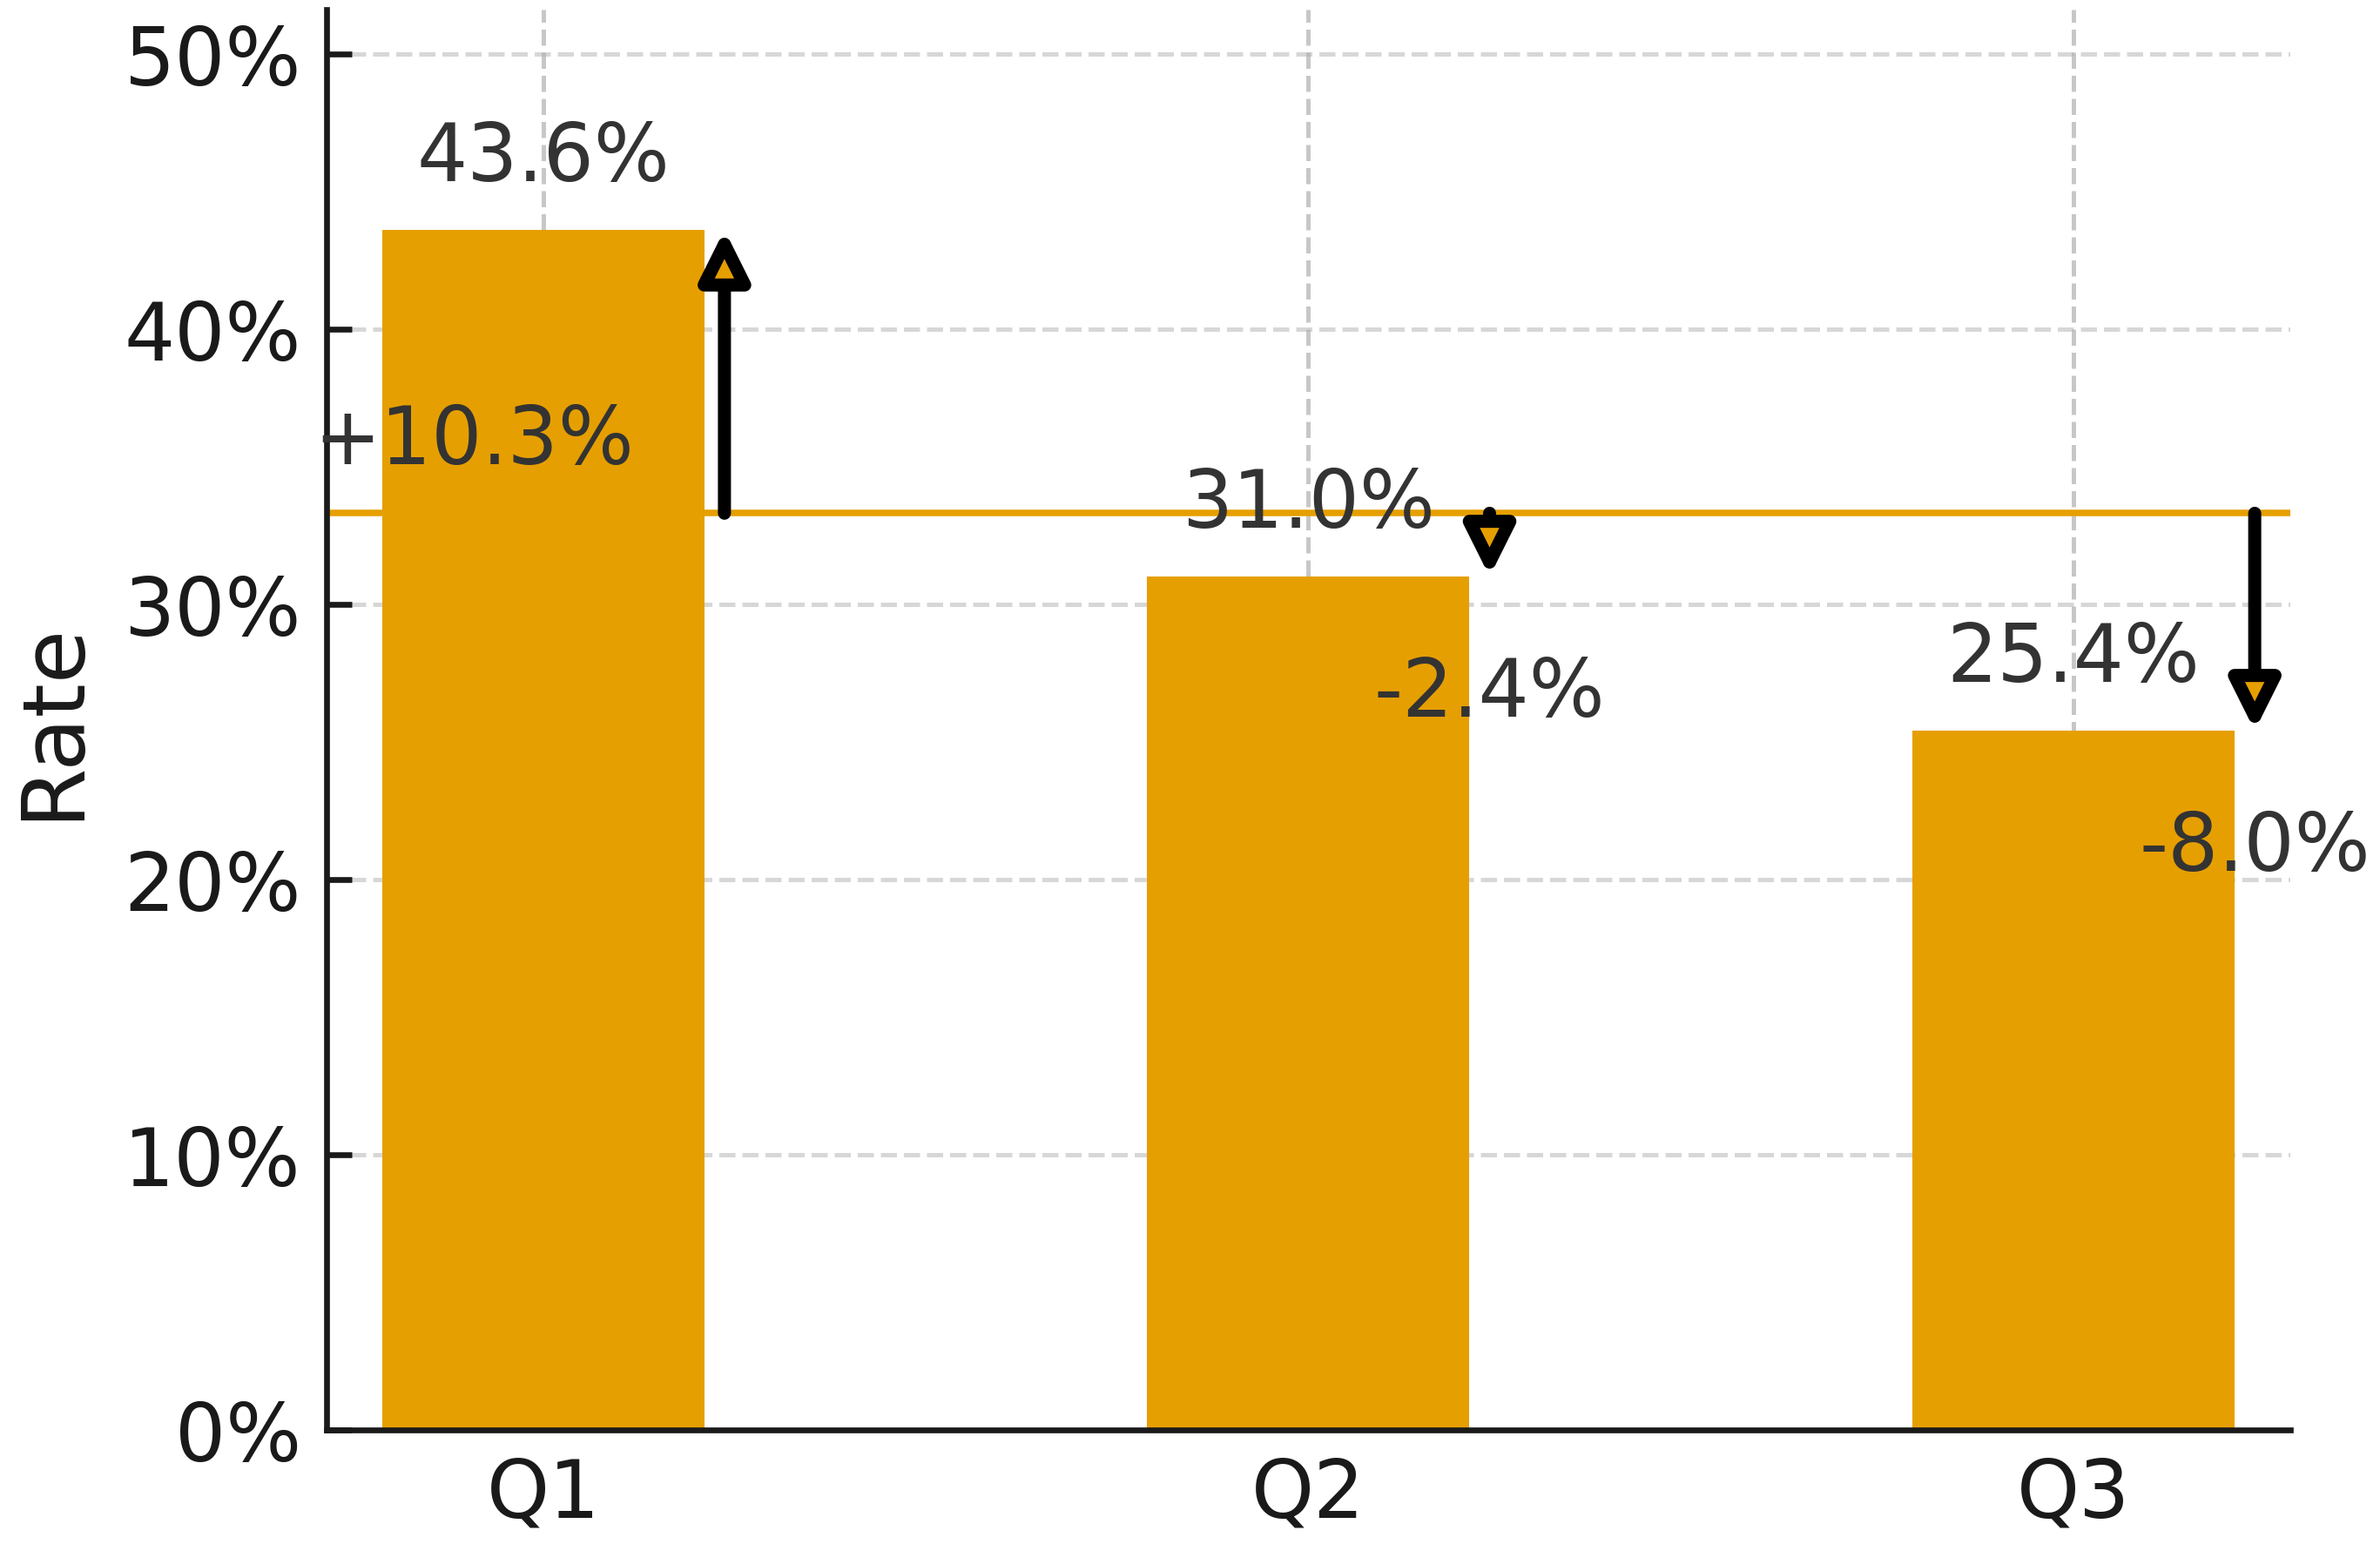
\includegraphics[]{figures/bias.png}}
    \end{minipage}
 \caption{\textbf{Data Distribution of Questions in} \ourdataset. (Left) Distribution of number of questions selected after filtering from articles (Right) We show the number of questions generated, and the proportion of the first, second and third generated question being picked as the final ``best question''.}
    \label{fig:databreakdown}
\end{figure}

As Figure \ref{fig:databreakdown} (left) illustrates, the generation process yielded mixed results. Post-processing, 39\% of source articles failed to produce any valid questions. Among the surviving articles, 21\% yielded exactly one valid question, which we retained. For the 61\% of articles producing multiple valid questions, we employed another LLM to identify the best candidate based on global relevance, specificity, and unambiguity. Our analysis of selected questions, shown in Figure \ref{fig:databreakdown} (right) reveals a selection bias:
\begin{itemize}
    \item Question 1: Selected 43.6\% of the time (10.3\% above random).
    \item Question 2: Selected 31\% of the time (2.4\% below random).
    \item Question 3: Selected 26.7\% of the time (6.7\% below random).
\end{itemize}
This trend suggests that initial generation attempts (question positioned earlier) frequently produce higher-quality results. Figure \ref{tab:succinct_forecasting_questions_v2} provides qualitative examples of these generated questions.

\begin{table}[h]
\centering
\resizebox{0.9\textwidth}{!}{%
\begin{tabular}{l*{10}{c}}
\toprule
 & \textbf{Name(s)} & \textbf{Location} & \textbf{Country} & \textbf{Title} & \textbf{Team} & \textbf{Color} & \textbf{Organization} & \textbf{Currency} & \textbf{Brand} & \textbf{Month} \\
 & & & & & \textbf{name} & & & & \textbf{name} & \\
\midrule
\textbf{Count} & 32{,}213 & 14{,}337 & 2{,}579 & 2{,}479 & 1{,}445 & 1{,}047 & 1{,}030 & 877 & 779 & 730 \\
\textbf{Share} & 44.8\% & 20.0\% & 3.6\% & 3.5\% & 2.0\% & 1.5\% & 1.4\% & 1.2\% & 1.1\% & 1.0\% \\
\bottomrule
\end{tabular}%
}
\caption{Top ten answer types of the questions in our curated dataset. These ten categories cover 80.1\% of our training dataset.}
\label{tab:answer_type_top10_horizontal}
\end{table}

\subsection{Distribution of Answer Types}
Table \ref{tab:answer_type_top10_horizontal} categorizes the answer types within the training data. Two categories dominate the dataset:
\begin{itemize}
    \item People and Places (65\%): Names of individuals constitute nearly 45\% of the answers, while locations account for 20\%.
    \item Miscellaneous Entities (35\%): The remainder consists of teams, countries, organizations, colors, and similar entities.
\end{itemize}

\begin{table}[h]
\centering
\small
\setlength{\tabcolsep}{4pt}
\renewcommand{\arraystretch}{1.2}
\begin{tabularx}{\textwidth}{L L L L L L}
\toprule
\textbf{Question} & \textbf{Background} & \textbf{Resolution (trigger \& deadline)} & \textbf{Answer Type} & \textbf{Answer} & \textbf{Source} \\
\midrule
Host country of COP30 (Nov 2025)? & UNFCCC COP venue rotates among regions. & Host confirmed by UNFCCC/organizers; no later than COP30 start (Nov 2025). & string (country) & Brazil & DW:\newline \href{https://www.dw.com/en/donald-trump-climate-policy-2025/a-71354256?maca=en-rss-en-all-1573-xml-atom}{link} \\
\midrule
Release month of Marvel's \emph{Fantastic Four} (2025)? & Reboot announced with lead cast; 2025 release slated. & Month confirmed by Marvel/Disney; by Dec 2025. & string (month) & July & Forbes:\newline \href{https://www.forbes.com/sites/caileygleeson/2024/02/16/x-men-fans-push-back-against-anger-over-non-binary-character/}{link} \\
\midrule
First state to require Ten Commandments in public classrooms (by 2025)? & Several U.S. states advance religion-in-school measures. & First state enacts requirement; by Dec 31, 2025. & string (state name) & Louisiana & Forbes:\newline \href{https://www.forbes.com/sites/maryroeloffs/2024/06/20/louisianas-new-ten-commandments-law-is-latest-example-of-states-pushing-to-allow-religion-in-public-schools/}{link} \\
\midrule
African host of G20 Summit (Nov 2025)? & G20 presidency rotates; South Africa presiding from Dec 2024. & G20/host government confirms location; by Nov 2025. & string (country) & South Africa & DW:\newline \href{https://www.dw.com/en/africa-in-2025-strengthening-democracy-key-to-growth/a-70945864}{link} \\
\midrule
Recipient of Lesotho--Botswana Transfer Scheme (by 2025)? & Regional pipeline to pump water from Lesotho via SA. & ORASECOM or governments confirm recipient; by 2025. & string (country name) & Botswana & DW:\newline \href{https://www.dw.com/en/lesotho-urged-to-compensate-villagers-for-water-projects/a-69352942}{link} \\
\bottomrule
\end{tabularx}
\caption{Five succinct forecasting questions spanning climate, entertainment, law, geopolitics, and infrastructure; selected for brevity and diverse sources (DW, Forbes). Each row lists the question (summarized here for conciseness), short background, resolution trigger with deadline, answer type, ground-truth answer, and citation.}
\label{tab:succinct_forecasting_questions_v2}
\end{table}



\subsection{Test Set}
\label{sec:test_set_details}

For the test set, we first prepare an initial set of 1000 questions generated using \texttt{o4-mini-high} model as described in \Cref{sec:results}. We next performed additional filtering steps to retain high-quality future-facing questions: 
\begin{enumerate}
    \item We removed any potentially unanswerable questions (noise) by keeping only those which \texttt{grok-4.1-fast} could successfully answer majority of the times (run repeatedly, $n=5$) with search tool access. This filtered out $15\%$ of the questions.
    \item To address the issue of late reporting in news outlets, we again use \texttt{grok-4.1-fast} with search tool to find the \textbf{earliest resolution date} for a given question. This is important to prevent leakage from retrieving articles with the true answer. We retain only those questions with resolution date after May 2025. In \Cref{fig:correct_resolution_date}, we report the number of questions per news source for whom the generated resolution date was within 1 month period of the date found by \texttt{grok-4.1-fast}. We notice an average of $70\%$ questions have resolution date even within the 1 month period. %This helps us estimate that around $30\%$ of the 
\end{enumerate} 

Finally, we manually filter the remaining questions to meet our quality checks like: 
\begin{enumerate}
    \item Question may have multiple possible correct answers. % like "
    \item Question actually resolves in the future (after September 2025) for which the article reports the scheduled/planned place/event/etc. % For example, 
    \item Question being irrelevant because it is too niche to a certain place or locality.
    \item Question is about something which is already established (known).
\end{enumerate}

We provide the full guidelines we followed for manual filtering in the box below. This resulted in a final test set of $302$ questions which we use for reporting the results.

\begin{figure}[b]
\vspace{-0.05cm}
    \centering

    % (a) left plot
    \begin{subfigure}[t]{0.49\textwidth}
        \centering
        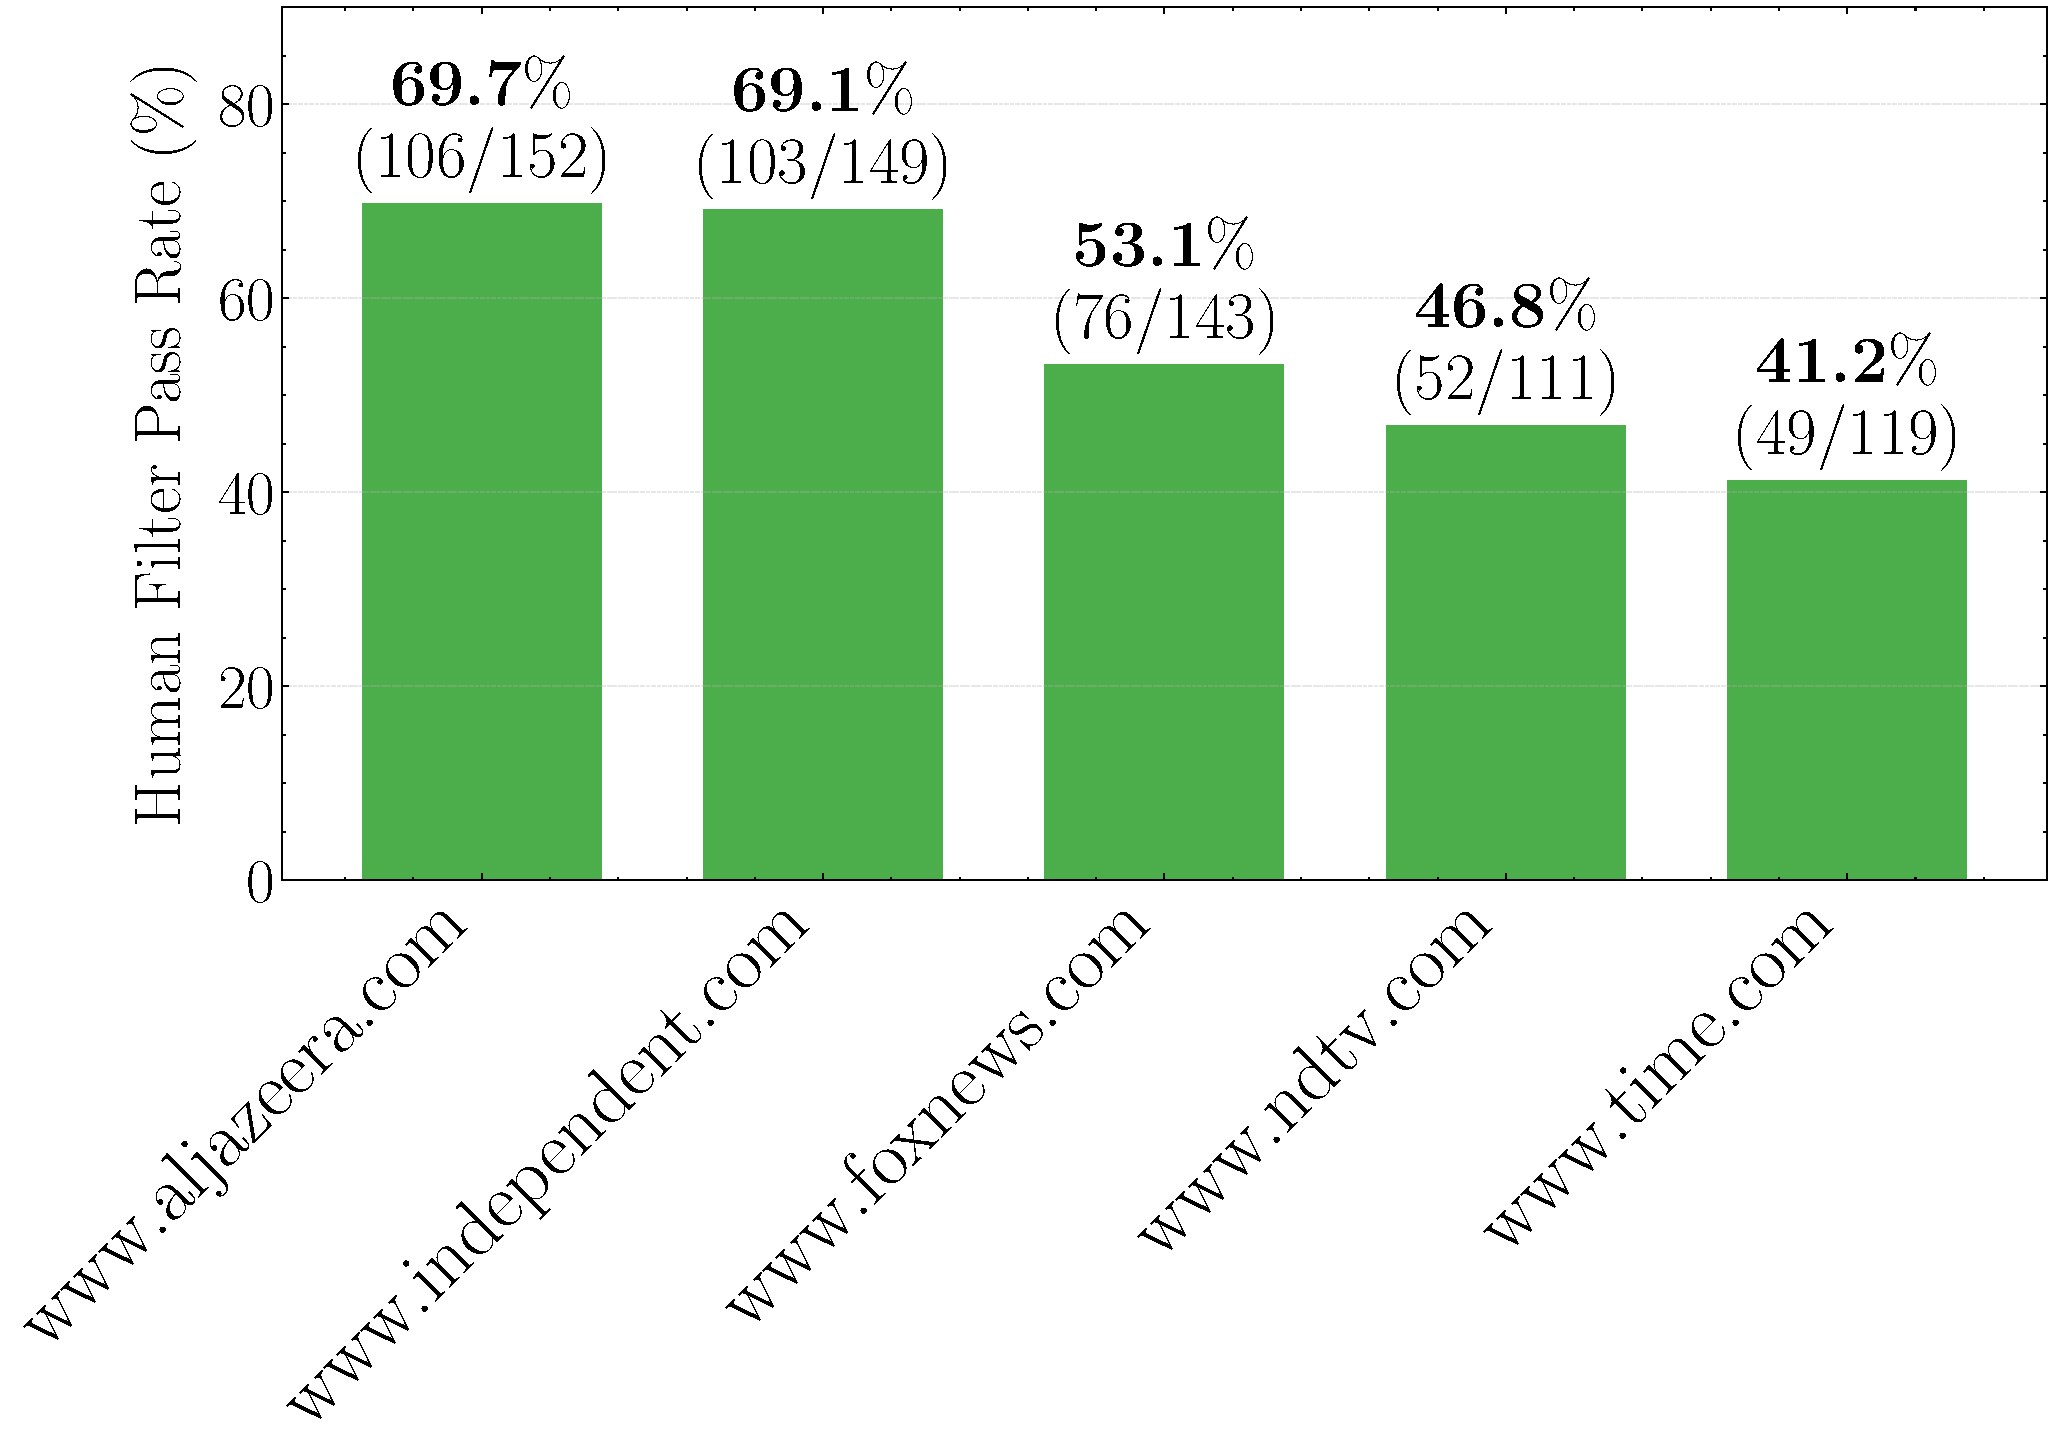
\includegraphics[width=0.95\linewidth]{figures/testset-final/filtering/human_pass_by_source.pdf}
        \caption{Manual filter pass rate per news source.}
        \label{fig:manual_filter_rate}
    \end{subfigure}
    \hfill
    % (b) right plot
    \begin{subfigure}[t]{0.49\textwidth}
        \centering
        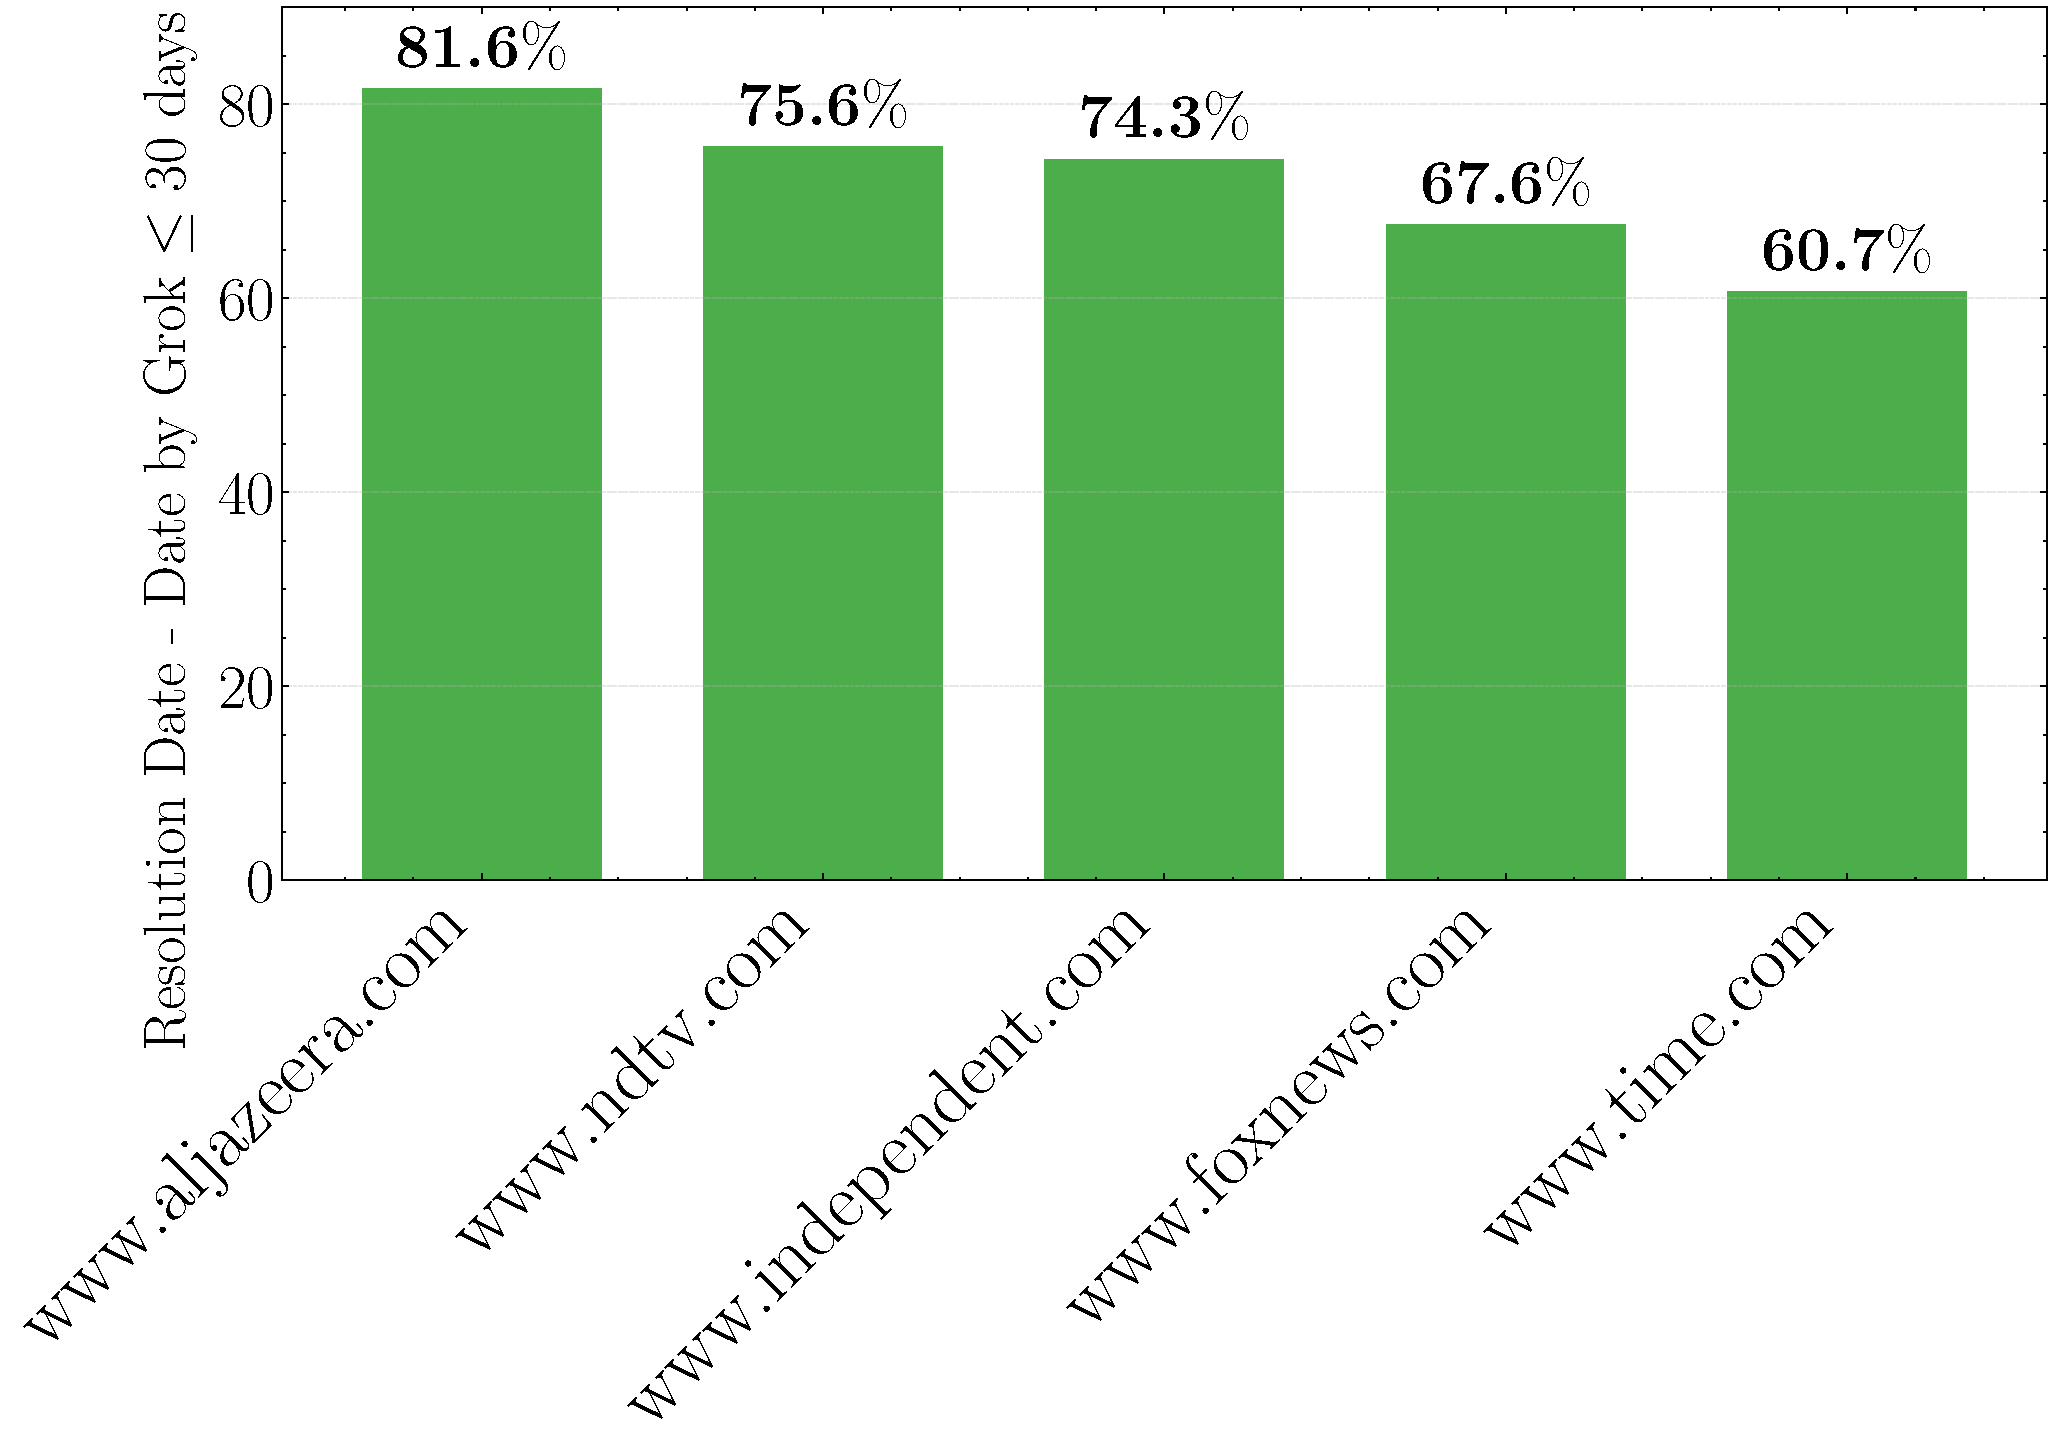
\includegraphics[width=0.95\linewidth]{figures/testset-final/filtering/late_resolution_30days_by_source.pdf}
        \caption{Proportion of questions whose resolution date is within 1 month of the resolution date found by grok-4.1-fast.}
        \label{fig:correct_resolution_date}
    \end{subfigure}

    \caption{
        Filtering pass rate of forecasting questions across news sources.
        }
    
    \vspace{-.4cm}
\end{figure}
% \clearpage

\begin{tcblisting}{
  title={\textbf{Manual Filtering Guidelines}},
  colframe=black!70,
  colback=black!2,
  boxrule=0.5pt,
  breakable,
  listing only
}
**Task:** You will be given (i) a news article and (ii) a question that is supposed to be answerable from that article. Your job is to decide whether to KEEP the question in the test set or REJECT it during manual filtering.

**How to review:**
1. Read the full question (Title, Background, Resolution Criteria, and the proposed Answer).
2. Apply the rejection criteria below. If **any** criterion triggers, REJECT the question. Refer to the article text if required.

------------------------------------------------------------
**REJECT the question if it fails ANY of the following criteria:**

1) **Multiple possible correct answers (Ambiguous / not uniquely resolvable)**
   - Reject if the question could reasonably have more than one correct answer, even after reading the article.
   - Examples:
     - "Which company invested in ABC in July 2025?" when multiple companies are mentioned investing in ABC in July 2025.
     - "Who announced a new partnership?" when the article lists several partnerships.

2) **Resolves in the future (after September 2025)**
   - Reject if the question's true resolution depends on an event that happens **after 2025-09-30**, and the article only reports a *plan/schedule/announcement* rather than the event actually occurring.
   - Examples:
     - Article: "The ABC event is scheduled for Jan 2026 in PQR venue."
       Question: "Where will event ABC be held in Jan 2026?" -> Reject (the question resolves only after the event actually takes place as the venue can change last minute).

3) **Too niche / overly local / low general relevance**
   - Reject if the question is narrowly tied to a very specific locality, institution, or small community such that it is not broadly meaningful for a general test set.
   - Examples:
     - A minor municipal policy affecting only one small village.
     - A local event with no wider regional/national/global significance.

4) **Already established (Known / not a meaningful forecast target)**
   - Reject if the question is about something that is already settled or widely known at the time (i.e., not an uncertain outcome).
   - Examples:
     - "Who stepped down from the role of CEO of Company ABC in August 2025?" (requires knowing the current CEO which generally doesn't change frequently and is often stable over multiple years)
     - Long-established facts, definitions, or historical constants.

------------------------------------------------------------
**Decision format (for annotation):**
- If any criterion triggers, then **REJECT**.
- Otherwise, **KEEP**.

**Question:**
{questions_text}

<toggle> **Source Article:** {source_article} </toggle>
\end{tcblisting}



\clearpage
